%
% lichtkegel.tex -- lichtkegel entlang einer Bahn in Finkelstein-Koorsdinaten
%
\documentclass[tikz]{standalone}
\usepackage{fp}
\usepackage{ifthen}
\usetikzlibrary{arrows,intersections}
\usetikzlibrary{fixedpointarithmetic}
\begin{document}
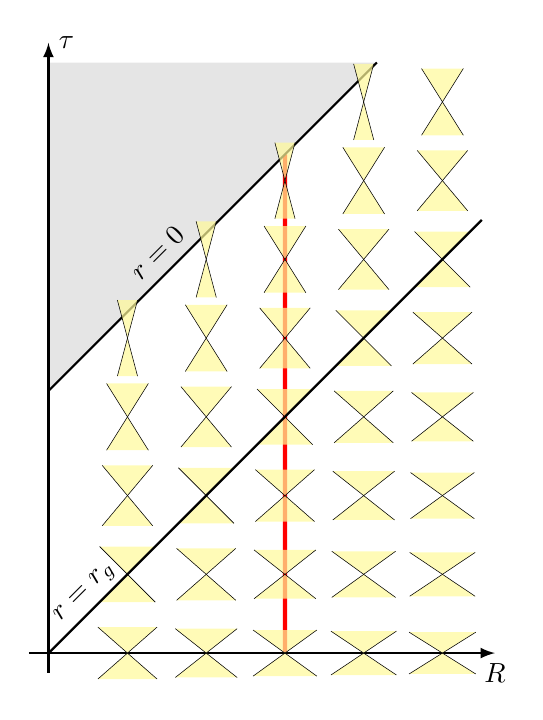
\begin{tikzpicture}[>=latex, thick, scale = 5, fixed point arithmetic]
\definecolor{lightconecolor}{cmyk}{0,0,1,0}
\coordinate (O) at (0.666,0);

\draw [line width = 1.5, red] (1.26666,0)--(1.2666,1.2666);
\fill[gray!20] (0.666,0.666) -- (1.50,1.50) -- (0.666,1.50)--cycle;
\draw[->] (0.616,0) -- (1.8,0) coordinate[label = {below:$R$}] (xmax);
\draw[->] (0.666,-0.05) -- (0.666,1.55) coordinate[label = {right:$\tau$}] (ymax);
\draw (0.666,0.666)--(1.50,1.50);

\def\s{0.1};
\newcommand\lightcone[2]{
\def\r{#1}
\def\t{#2}
\pgfmathsetmacro{\angle}{45 + 1.5 * (atan(((3/2) * (\r - \t))^(1/3)) - 45)}
\fill[lightconecolor!40, opacity = 0.7] ({\r + \s * sin(\angle)}, {\t + \s * cos(\angle)})
            -- ({\r}, {\t})
            -- ({\r - \s * sin(\angle)}, {\t + \s * cos(\angle)})
            -- cycle;
\fill[lightconecolor!40, opacity = 0.7] ({\r - \s * sin(\angle)}, {\t - \s * cos(\angle)})
            -- ({\r}, {\t})
            -- ({\r + \s * sin(\angle)}, {\t - \s * cos(\angle)})
            --cycle;
\draw [very thin] ({\r + \s * sin(\angle)}, {\t + \s * cos(\angle)})
   -- ({\r - \s * sin(\angle)}, {\t - \s * cos(\angle)});
\draw  [very thin]({\r + \s * sin(\angle)}, {\t - \s * cos(\angle)})
   -- ({\r - \s * sin(\angle)}, {\t + \s * cos(\angle)});
}

\foreach \h in {4,...,8} {
	\foreach \v in {0,...,\h} {
		{\ifthenelse{\NOT 8 = \v}{
			\lightcone{0.06666 + 0.2 * \h}{0.2 * \v}
		}{}};
	}
}
\draw (0.6666,0)--(1.7666,1.1);
\node [label={[rotate=45] $r=0$}] at (0.976,0.956) {};
\node [label={[rotate=45] $r=r_g$}] at (0.796,0.09) {};



%\lightcone{1}{1.1}

\end{tikzpicture}
\end{document}

